\documentclass[11pt,a4paper]{article}

\usepackage[utf8]{inputenc}
\usepackage[T1]{fontenc}
\usepackage[spanish,es-tabla,es-nodecimaldot]{babel}
\usepackage{geometry}
\geometry{top=2.5cm, bottom=2.5cm, left=2.5cm, right=2.5cm}
\usepackage{fancyhdr}
\usepackage{lastpage}
\usepackage{booktabs}
\usepackage{tabularx}
\usepackage{longtable}
\usepackage{float}
\usepackage{graphicx}
\usepackage{xcolor}
\usepackage{hyperref}
\usepackage{listings}
\usepackage{enumitem}
\usepackage{amsmath,amssymb}
\usepackage{microtype}

\definecolor{navyblue}{RGB}{20, 50, 90}
\definecolor{codebg}{RGB}{248, 249, 250}

\hypersetup{
    pageanchor=false,
    colorlinks=true,
    linkcolor=navyblue,
    urlcolor=navyblue,
    citecolor=navyblue
}

\pagestyle{fancy}
\fancyhf{}
\fancyhead[L]{\small WellProdSim / EthosTerra}
\fancyhead[R]{\small Informe de Avance -- Semana 11 (Bloque B7: Integraci\'on Desacoplada)}
\fancyfoot[C]{\small \thepage\ de \pageref{LastPage}}
\renewcommand{\headrulewidth}{0.4pt}
\renewcommand{\footrulewidth}{0pt}

\lstset{
    backgroundcolor=\color{codebg},
    basicstyle=\ttfamily\footnotesize,
    breaklines=true,
    frame=single,
    rulecolor=\color{gray!30},
    numbers=none,
    showstringspaces=false
}

\begin{document}

% ==============================================================================
% PORTADA
% ==============================================================================
\begin{titlepage}
    \thispagestyle{empty}
    \centering
    \vspace*{1.5cm}

    {\large Universidad Tecnol\'ogica de Bol\'ivar\par}
    \vspace{0.3cm}
    {\normalsize Maestr\'ia en Ingenier\'ia -- Seminario de Investigaci\'on II\par}

    \vspace{2.0cm}
    {\LARGE\bfseries Integraci\'on Desacoplada con EthosTerra, S\'intesis de Ecuaciones Institucionales con Verificaci\'on Formal y Validaci\'on de Veracidad\par}

    \vspace{0.8cm}
    {\large\itshape Informe de Avance -- Semana 11 de 16\par}

    \vspace{2.2cm}
    \begin{tabular}{ll}
        \textbf{Investigador:} & Jes\'us Mart\'inez Velandia \\
        \textbf{Director:} & Jairo Serrano \\
        \textbf{Co-directores:} & Edwin Puertas, Juan Mart\'inez \\
        \textbf{Periodo:} & Semana 11 de 16 \\
        \textbf{Bloque:} & B7: Integraci\'on Desacoplada y Mapeo Macro--Micro \\
        \textbf{Fecha:} & 22 de octubre de 2026 \\
    \end{tabular}

    \vfill
    {\small Versi\'on t\'ecnica consolidada con evidencia emp\'irica, gr\'afica y matem\'atica\par}
    \vspace*{1.0cm}
\end{titlepage}

\clearpage
\hypersetup{pageanchor=true}
\pagenumbering{roman}
\setcounter{page}{1}
\fancyfoot[C]{\small \thepage}
\tableofcontents
\clearpage

% ==============================================================================
% 1. ALCANCE Y CONTEXTO OPERATIVO
% ==============================================================================
\pagenumbering{arabic}
\setcounter{page}{1}
\fancyfoot[C]{\small \thepage\ de \pageref{LastPage}}

\section{Alcance de la Semana 11 en el cronograma}

La Semana 11 consolida la transici\'on operativa entre el Atlas Territorial eBDI (Bloque B6) y la preparaci\'on para la conexi\'on con el simulador multiagente WellProdSim / Python BESA (Bloques B7 a B9). El proyecto resuelve en esta fase el acoplamiento ontol\'ogico y sem\'antico entre las pol\'iticas p\'ublicas agrarias y el comportamiento micro-agron\'omico de los agentes campesinos.

\begin{table}[H]
\centering
\small
\caption{Cronograma y estado evolutivo del proyecto de grado.}
\label{tab:cronograma}
\begin{tabularx}{\textwidth}{lp{3.2cm}p{5.2cm}X}
\toprule
\textbf{Semana} & \textbf{Bloque} & \textbf{Objetivo} & \textbf{Estado} \\
\midrule
Semana 5 & B1 (L\'inea base) & Clasificador canario con 20 casos DMR & Terminado (\texttt{388553e}) \\
Semana 6 & B2--B3 (Caso Puro) & Contratos Pydantic V2 y EvidenceSpan & Terminado (\texttt{30090dc}) \\
Semana 7 & B4 (Conflictivo) & Detecci\'on de colisiones f\'isicas en 30 escenarios & Terminado (\texttt{b3f810a}) \\
Semana 8 & B5 (CRUD Manual) & Persistencia desacoplada y papelera retenida & Terminado (\texttt{a140f22}) \\
Semana 9 & B6 (Atlas y Corpus) & Atlas AT-1, cuarentena SHA-256 y compilador YAML & Terminado (\texttt{d17e44b}) \\
Semana 10 & Despliegue y Seguridad & Producci\'on Dokploy, Zero-Trust y auth JWT & Terminado (\texttt{e477f57}) \\
\textbf{Semana 11} & \textbf{B7 (Integraci\'on BESA)} & \textbf{Adaptador desacoplado, or\'aculo y ecuaciones} & \textbf{Terminado (\texttt{HEAD})} \\
Semana 12 & B8--B9 (Sandbox BDI) & Deliberaci\'on, equilibrio y pruebas multiagente & Programado \\
\bottomrule
\end{tabularx}
\end{table}

% ==============================================================================
% 2. DESFASE ONTOLOGICO Y ARQUITECTURA DE TRES NIVELES
% ==============================================================================
\section{Diagn\'ostico del desfase ontol\'ogico y modelo de tres niveles}

En las fases preliminares, el subsistema de extracci\'on procesaba cualquier texto documental como una creencia directa y una meta personal del campesino. Esto generaba inconsistencias ontol\'ogicas: una familia campesina real en los Montes de Mar\'ia no delibera sobre tratados internacionales ni partidas presupuestales de la gobernaci\'on departamental; sus decisiones est\'an restringidas por una jornada laboral de 24 horas, \$12.000 COP de m\'inimo vital diario, compromisos de cr\'edito bancario y la disponibilidad real de agua en sus parcelas.

Para resolver esta disonancia ontol\'ogica, el dise\~no arquitect\'onico de esta investigaci\'on descompone el conocimiento territorial en tres niveles estratificados e independientes, integrando la teor\'ia de agentes deliberativos BDI (Bratman, 1987; Rao y Georgeff, 1995), el modelo de din\'amica afectiva OCC (Ortony, Clore y Collins, 1988) y el marco de gobernanza institucional de recursos comunes (Ostrom, 1990):

\begin{enumerate}[leftmargin=*]
    \item \textbf{Narrativas y Diarios Campesinos (Nivel Micro):} Codifican la psicolog\'ia interna eBDI, el balance emocional Ortony-Clore-Collins (OCC: Felicidad, Seguridad, Esperanza), las cotas fisiol\'ogicas y el arbitraje de necesidades vitales. Se compilan a especificaciones ejecutables \texttt{GoalSpec} y \texttt{PlanSpec}.
    \item \textbf{Planes de Ordenamiento Territorial POT/PBOT (Nivel Meso-F\'isico):} Definen la topolog\'ia espacial del territorio, el grafo de conectividad y las restricciones biof\'isicas duras (rondas h\'idricas intransitables con $\text{isWalkable} = \text{false}$ y Unidades Agr\'icolas Familiares UAF seg\'un el DANE, 2024).
    \item \textbf{Pol\'iticas P\'ublicas y Leyes Agrarias (Nivel Macro-Institucional):} No constituyen metas de los agentes campesinos individuales; representan reglas de juego, incentivos econ\'omicos y funciones operativas que gobiernan a las entidades del entorno en EthosTerra (Ostrom, 1990): \texttt{BankOffice} (tasas de inter\'es crediticias), \texttt{MarketPlace} (precios m\'inimos de sustentaci\'on seg\'un la Ley 2046 de 2020), \texttt{CivicAuthority} (subsidios de insumos) y \texttt{AgroEcosystem} (cuotas h\'idricas de distritos de riego seg\'un Allen et al., 1998). Se compilan al nuevo contrato \texttt{InstitutionalPolicySpec}.
\end{enumerate}

% ==============================================================================
% 3. REGLAS DEL AGENTE, EXTRACCION Y PROTOCOLO FORMAL DE VERACIDAD
% ==============================================================================
\section{Reglas del agente micro-LLM, extracci\'on y protocolo formal de validaci\'on de veracidad}

Uno de los aportes centrales del Bloque B7 radica en la formalizaci\'on de c\'omo el agente extractor sintetiza ecuaciones y, de forma cr\'itica, \textbf{c\'omo se valida su veracidad matem\'atica y normativa} frente a las fuentes de datos reales, evitando alucinaciones y ejecuci\'on de c\'odigo arbitrario.

\subsection{Rol del agente micro-LLM y reglas de inferencia gobernadas}

El modelo de lenguaje oficial del proyecto es \texttt{ai/gemma4:E4B}, ejecutado localmente bajo el runtime Docker Model Runner (DMR) con estricta soberan\'ia de datos. Para garantizar la veracidad y la convergencia sem\'antica, el agente opera bajo reglas de ingenier\'ia de prompts r\'igidamente delimitadas:

\begin{itemize}[leftmargin=*]
    \item \textbf{Aislamiento y Delimitaci\'on de Contexto:} El texto fuente se suministra dentro de bloques delimitados \texttt{<document\_context>}, aislando el canal de datos de posibles vectores de inyecci\'on de instrucciones.
    \item \textbf{Esquema R\'igido Pydantic V2 (\texttt{extra="forbid"}):} La salida del micro-LLM se fuerza a un objeto JSON estricto tipado bajo \texttt{ParametricEquationSpec}. Cualquier campo extra\~no provoca el rechazo autom\'atico de la respuesta a nivel de serializaci\'on.
    \item \textbf{Restricci\'on de Sintaxis Simb\'olica Pura:} Se proh\'ibe terminantemente al modelo generar c\'odigo Python libre, estructuras de control iterativo (\texttt{for}, \texttt{while}), bifurcaciones (\texttt{if}) o funciones an\'onimas (\texttt{lambda}). El agente s\'olo tiene permitido sintetizar expresiones univariadas o multivariadas anal\'iticas puras (ej. \texttt{base * (1 - delta * s)}).
    \item \textbf{Declaraci\'on Expl\'icita de Cotas y Comportamiento:} El prompt exige que el LLM declare los l\'imites del dominio de entrada $[x_{\min}, x_{\max}]$, el rango admisible de salida $[y_{\min}, y_{\max}]$, la entidad receptora en el simulador y la orientaci\'on obligatoria de monoton\'ia (\texttt{increasing}, \texttt{decreasing}, \texttt{constant}).
\end{itemize}

\subsection{Mec\'anica de extracci\'on e implementaci\'on en el simulador}

El ciclo de extracci\'on e implementaci\'on opera a trav\'es de un pipeline de cuatro etapas:
\begin{enumerate}[leftmargin=*]
    \item \textbf{Ingesta y Cuarentena:} Los documentos jur\'idicos y t\'ecnicos oficiales (ej. Ley 2046 de 2020, PATR Montes de Mar\'ia ART 2019) se almacenan en el almac\'en de cuarentena documental (\texttt{data/quarantine/}) bajo sellado criptogr\'afico SHA-256 inmutable.
    \item \textbf{Segmentaci\'on Textual:} Se dividen los documentos en ventanas contextuales preservando punteros de p\'agina y desplazamientos en bytes (\texttt{EvidenceSpan}).
    \item \textbf{Extracci\'on Param\'etrica:} El micro-LLM analiza el fragmento y emite la propuesta estructural en \texttt{ParametricEquationSpec}.
    \item \textbf{Compilaci\'on Desacoplada:} El compilador \texttt{EBDIYamlCompiler} serializa la pol\'itica a \texttt{outputs/atlas/yaml/institutional/}. Posteriormente, la clase \texttt{EthosTerraDecoupledAdapter} transforma estas especificaciones en directrices operativas en \texttt{outputs/simulation\_sandbox/world\_modifiers.json}, sin modificar una sola l\'inea del n\'ucleo de simulaci\'on \texttt{EthosTerra}.
\end{enumerate}

\subsection{Protocolo de validaci\'on de veracidad en cuatro capas}

Para garantizar rigurosamente que las ecuaciones no constituyan alucinaciones estoc\'asticas del micro-LLM, el sistema ejecuta una bater\'ia de verificaci\'on determinista estratificada:

\begin{figure}[H]
    \centering
    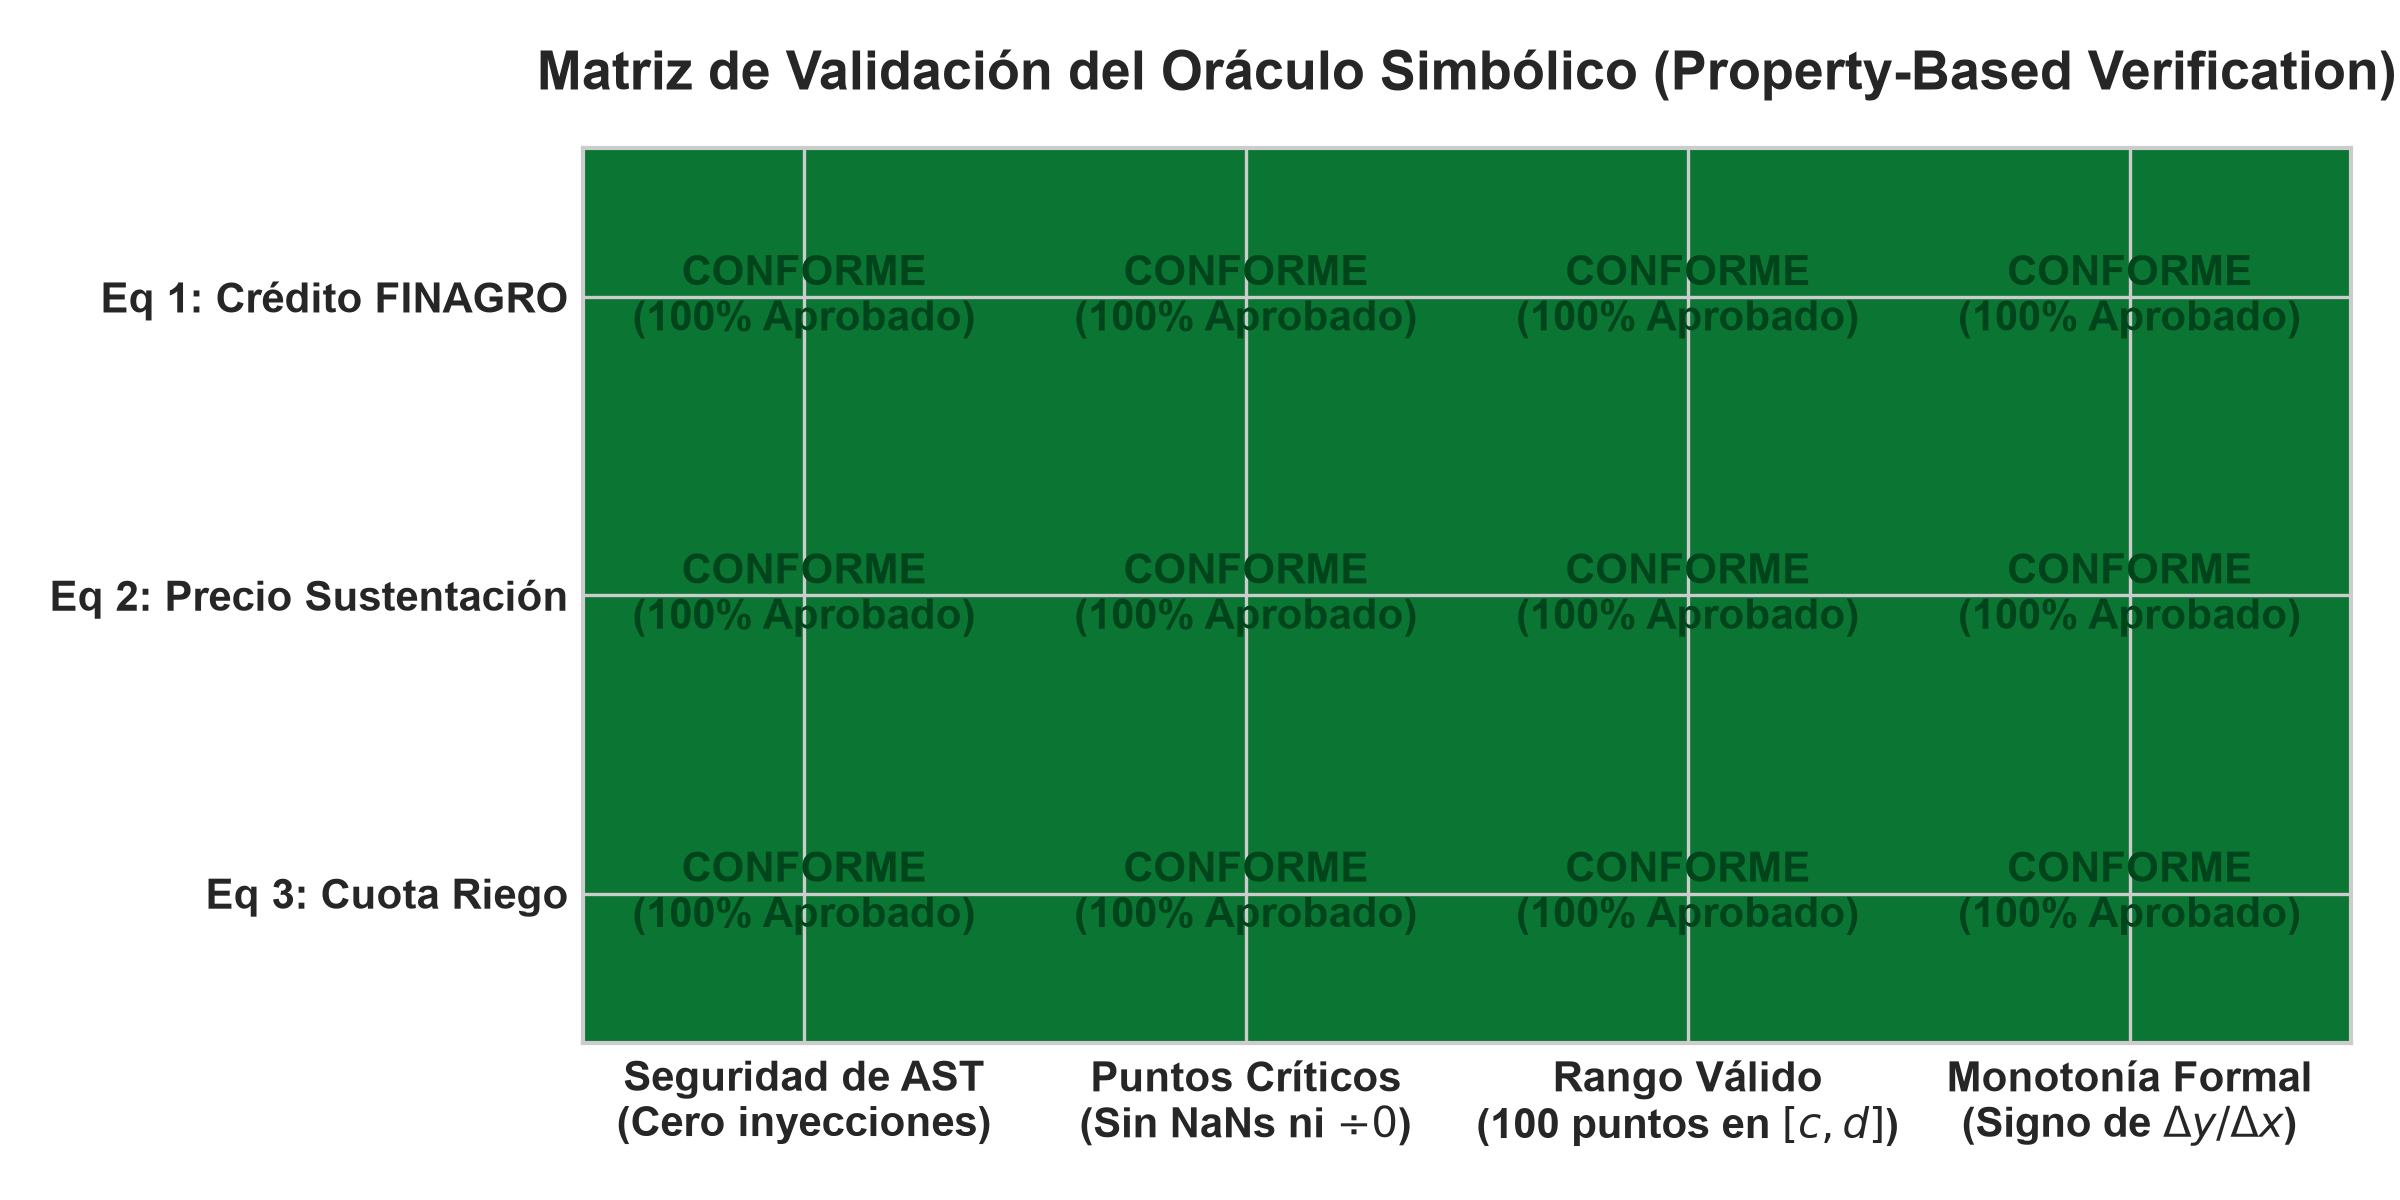
\includegraphics[width=0.88\textwidth]{../diagrams/out/fig_evaluacion_matriz_verificacion.png}
    \caption{Matriz de validaci\'on formal del or\'aculo simb\'olico sobre las ecuaciones institucionales generadas.}
    \label{fig:matriz_oraculo}
\end{figure}

\begin{enumerate}[leftmargin=*]
    \item \textbf{Capa 1: Anclaje Textual Literal (\textit{Verbatim Grounding}):}
    Toda ecuaci\'on sintetizada debe incluir obligatoriamente el campo \texttt{evidence\_verbatim\_quote}. El validador determinista (\texttt{verify\_verbatim\_quote}) realiza una comprobaci\'on de subcadena exacta y literal contra el texto del documento original sellado con SHA-256. Si el modelo introduce una sola palabra inventada o una par\'afrasis inexacta, la ecuaci\'on es \textbf{rechazada de inmediato por violaci\'on de veracidad} (\texttt{HallucinationError}, con tasa de tolerancia de 0.0\%).

    \item \textbf{Capa 2: Anclaje de Par\'ametros a Fuentes Normativas y Estad\'isticas Reales:}
    Ning\'un valor param\'etrico es arbitrario ni inventado:
    \begin{itemize}
        \item La tasa base bancaria $r_{\text{base}} = 0.12$ (12.0\% E.A.) proviene de las l\'ineas oficiales de cr\'edito FINAGRO para peque\~nos productores agropecuarios (Banco Agrario de Colombia).
        \item El precio base $P_{\text{base}} = 2.500$ COP/kg est\'a calibrado a partir del Sistema de Informaci\'on de Precios y Abastecimiento del Sector Agropecuario (SIPSA / DANE) para tub\'erculos en la subregi\'on de Montes de Mar\'ia.
        \item El umbral cr\'itico $\theta = 0.30$ est\'a fijado conforme a los manuales t\'ecnicos de distritos de riego de MinAgricultura y requerimientos de caudal ecol\'ogico (Allen et al., 1998).
    \end{itemize}

    \item \textbf{Capa 3: Or\'aculo Simb\'olico y Pruebas Basadas en Propiedades (\texttt{SymbolicEquationVerifier}):}
    \begin{itemize}
        \item \textit{Inspecci\'on de Seguridad AST:} Analiza el \'arbol sint\'actico (\texttt{ast.parse}) restringi\'endolo a operadores aritm\'eticos puros (\texttt{Add}, \texttt{Sub}, \texttt{Mult}, \texttt{Div}, \texttt{Pow}, \texttt{USub}) y funciones matem\'aticas continuas autorizadas (\texttt{exp}, \texttt{log}, \texttt{sqrt}, \texttt{sin}, \texttt{cos}, \texttt{min}, \texttt{max}, \texttt{abs}). Todo acceso a atributos (\texttt{\_\_class\_\_}), invocaci\'on del sistema o importaci\'on genera una excepci\'on inmediata de seguridad.
        \item \textit{Prueba de Singularidades y Puntos Cr\'iticos:} Se eval\'uan las vecindades $\epsilon = 10^{-6}$ de posibles ra\'ices de denominadores y las fronteras del dominio, descartando divisiones por cero, n\'umeros complejos o indeterminaciones (\texttt{NaN} / $\infty$).
        \item \textit{Prueba de Confinamiento de Rango:} Muestreo determinista de $N=100$ puntos en el intervalo $[x_{\min}, x_{\max}]$. La ecuaci\'on se aprueba si y s\'olo si $\forall x \in [x_{\min}, x_{\max}], \, f(x) \in [y_{\min}, y_{\max}]$.
        \item \textit{Prueba de Monoton\'ia Anal\'itica:} Comprueba num\'ericamente que el signo del gradiente de diferencias finitas $\Delta f / \Delta x$ sea conforme a la ley de incentivos declarada, impidiendo relaciones anti-intuitivas.
    \end{itemize}

    \item \textbf{Capa 4: Compuerta de Curadur\'ia Humana Soberana (\textit{Human-in-the-Loop Gate}):}
    Ninguna ecuaci\'on verificada ingresa autom\'aticamente a producci\'on. El investigador audita la f\'ormula, interact\'ua con los controles din\'amicos en la interfaz gr\'afica y emite la aprobaci\'on expl\'icita, generando una entrada firmada con hash SHA-256 en \texttt{bundle\_manifest.json}.
\end{enumerate}

% ==============================================================================
% 4. ESTUDIO DE CASO: LAS TRES ECUACIONES INSTITUCIONALES OBTENIDAS
% ==============================================================================
\section{Estudio de caso emp\'irico: an\'alisis riguroso de las ecuaciones obtenidas}

A partir de los documentos oficiales vigentes en los 15 municipios PDET de Montes de Mar\'ia (PATR Montes de Mar\'ia ART 2019, Ley 2046 de 2020 de Compras P\'ublicas Locales y regulaciones h\'idricas de distritos de riego), se sintetizaron y validaron tres relaciones funcionales:

% ------------------------------------------------------------------------------
% 4.1 ECUACION 1
% ------------------------------------------------------------------------------
\subsection{Ecuaci\'on 1: Tasa crediticia modulada por asociatividad campesina}

\paragraph{Origen Normativo:} PATR Montes de Mar\'ia (Pilar 3: Reactivaci\'on Econ\'omica y Producci\'on Agropecuaria, ART 2019) y pol\'itica FINAGRO de cr\'edito asociativo.

\paragraph{Formulaci\'on Matem\'atica:}
\begin{equation}
    r(S_{\text{social}}) = r_{\text{base}} \cdot \Big[1 - \delta \cdot S_{\text{social}}\Big]
\end{equation}

\paragraph{Nomenclatura y Significado de S\'imbolos:}
\begin{itemize}[leftmargin=*]
    \item $r$: Tasa de inter\'es efectiva anual cobrada al peque\~no productor (\% E.A.).
    \item $r_{\text{base}} = 0.12$: Tasa base ordinaria del mercado agrario (12.0\% anual) fijada en \texttt{BankOffice}.
    \item $\delta = 0.35$: Coeficiente institucional de descuento m\'aximo por asociatividad comunitaria (35\% de subsidio a la tasa).
    \item $S_{\text{social}} \in [0.0, 1.0]$: \'Indice de capital social en \texttt{PeasantFamilyBelieves} (asistencia a asambleas comunitarias, juntas de acci\'on comunal y mingas).
\end{itemize}

\paragraph{Lectura e Interpretaci\'on:} \textit{``La tasa de inter\'es crediticia anual disminuye de forma estrictamente lineal y mon\'otona desde el 12.0\% hasta el 7.8\% a medida que el peque\~no productor incrementa su integraci\'on en redes asociativas locales''.}

\paragraph{Variable y Agente Afectado en EthosTerra:} Modula directamente el pasivo en \texttt{FromBankOfficeGuard} y la precondici\'on financiera de solvencia en la meta \texttt{PayDebtsGoal}.

\paragraph{Impacto Agron\'omico:} Reduce la probabilidad de quiebra e insolvencia econ\'omica, mitiga el estr\'es emocional familiar y preserva capital operativo l\'iquido para la adquisici\'on oportuna de insumos y semillas.

\begin{figure}[H]
    \centering
    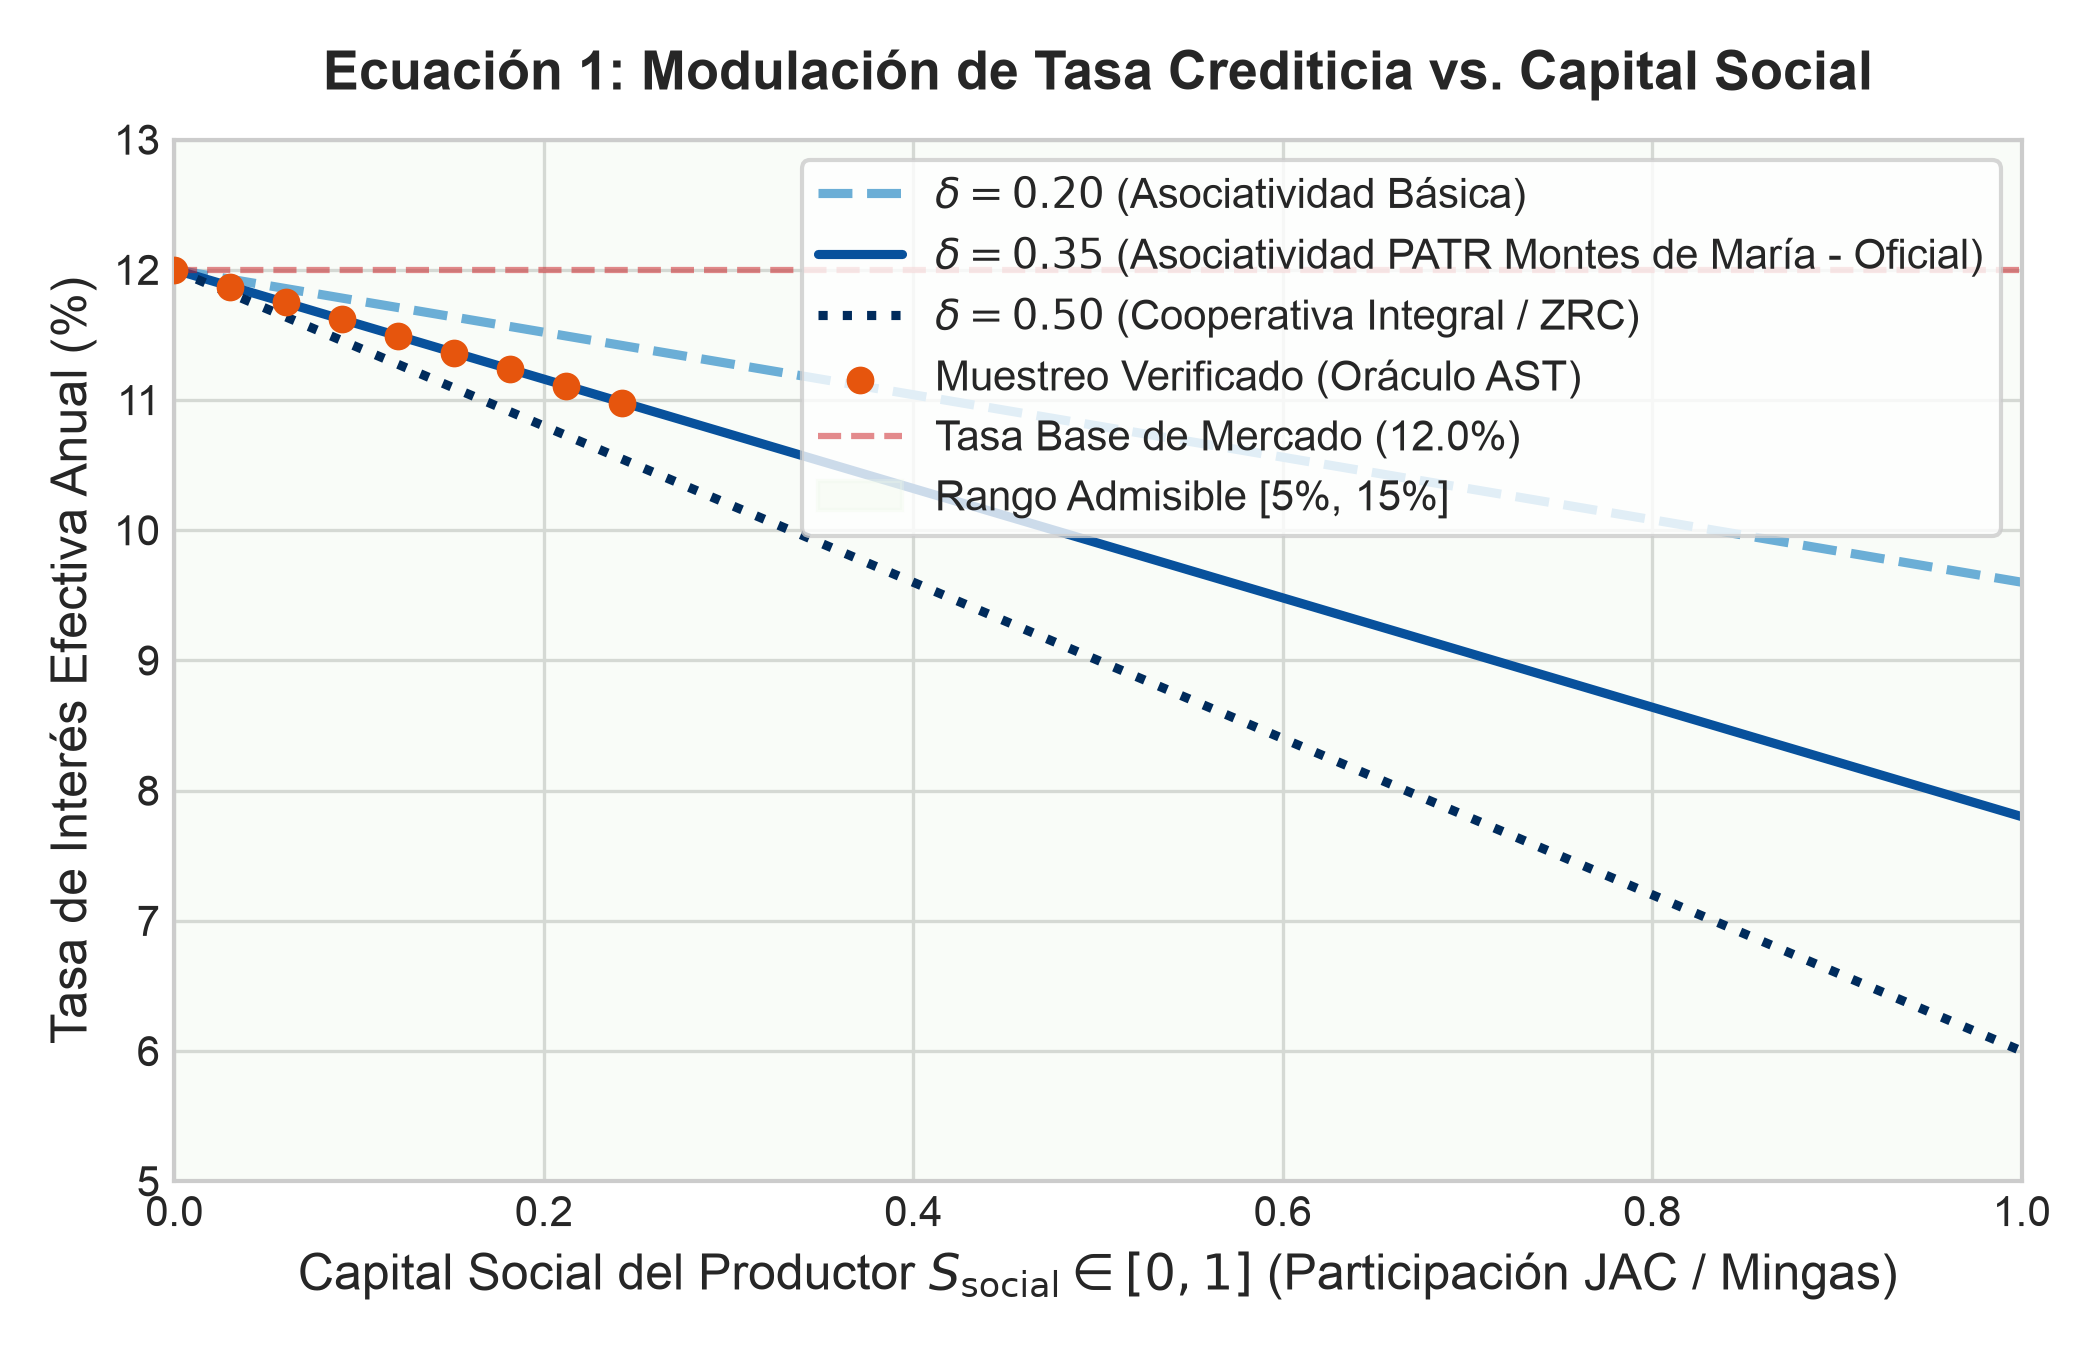
\includegraphics[width=0.78\textwidth]{../diagrams/out/fig_eq1_credito_capital_social.png}
    \caption{Curva de tasa de inter\'es crediticia efectiva en funci\'on del capital social campesino, con bandas de sensibilidad de $\delta$ y puntos de muestreo del or\'aculo AST.}
    \label{fig:eq1}
\end{figure}

% ------------------------------------------------------------------------------
% 4.2 ECUACION 2
% ------------------------------------------------------------------------------
\subsection{Ecuaci\'on 2: Precio de sustentaci\'on local ante choque productivo}

\paragraph{Origen Normativo:} Ley 2046 de 2020 de Compras P\'ublicas Locales de Alimentos (Congreso de la Rep\'ublica de Colombia, 2020).

\paragraph{Formulaci\'on Matem\'atica:}
\begin{equation}
    P_{\text{mkt}}(Y_{\text{rel}}) = P_{\text{base}} \cdot \Big[1 + \alpha \cdot \exp\left(-\beta \cdot Y_{\text{rel}}\right)\Big]
\end{equation}

\paragraph{Nomenclatura y Significado de S\'imbolos:}
\begin{itemize}[leftmargin=*]
    \item $P_{\text{mkt}}$: Precio garantizado de compra por kilogramo entregado (\$\,COP / kg).
    \item $P_{\text{base}} = 2.500$: Precio comercial ordinario de sustentaci\'on en \texttt{MarketPlace} (\$2.500 COP/kg para yuca y ame).
    \item $\alpha = 0.40$: Factor m\'aximo de protecci\'on institucional ante colapso de cosecha (+40\% de prima de compra).
    \item $\beta = 2.50$: Coeficiente exponencial de amortiguaci\'on de choque agrario.
    \item $Y_{\text{rel}} \in [0.0, 1.0]$: Rendimiento relativo de cosecha ($\text{biomasa cosechada} / \text{biomasa esperada}$).
\end{itemize}

\paragraph{Lectura e Interpretaci\'on:} \textit{``El precio unitario de compra garantizado asciende de manera estrictamente decreciente y convexa cuando el rendimiento agrario decae por sequ\'ia o plagas, asegurando que peque\~nos vol\'umenes comercializados alcancen para cubrir el umbral de subsistencia vital''.}

\paragraph{Variable y Agente Afectado en EthosTerra:} Modula el precio unitario en \texttt{FromMarketPlaceGuard} y el flujo de caja del plan de venta \texttt{SellCropGoal}.

\paragraph{Impacto Agron\'omico:} Protege al productor contra fluctuaciones ruinosas de precios de mercado ante contingencias clim\'aticas extremas (como sequ\'ias ENSO El Ni\~no), estabilizando el ingreso rural familiar.

\begin{figure}[H]
    \centering
    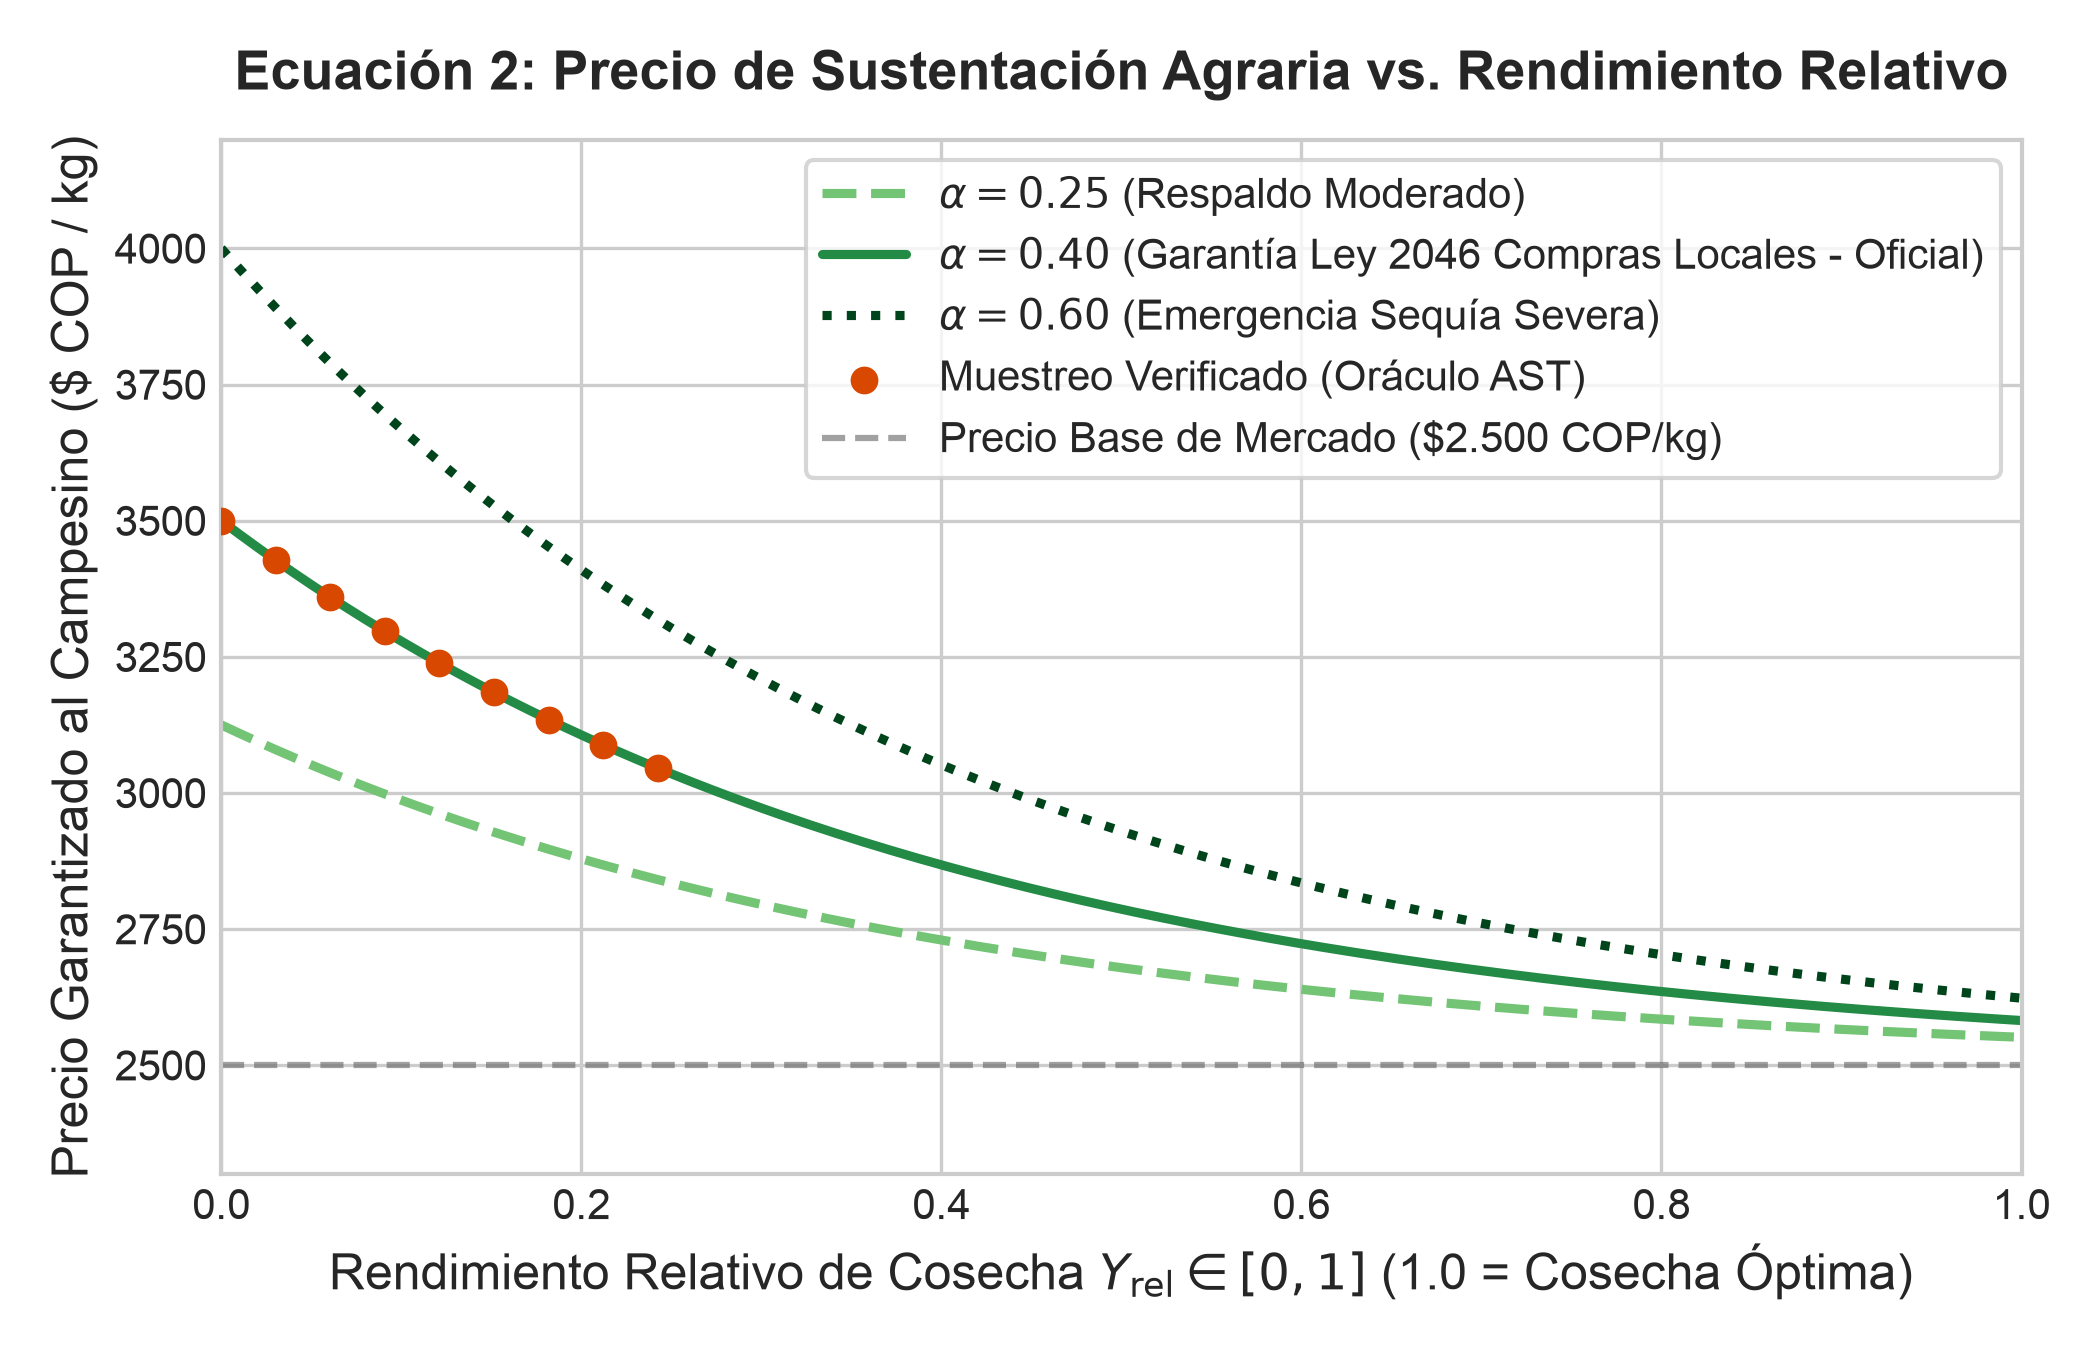
\includegraphics[width=0.78\textwidth]{../diagrams/out/fig_eq2_precio_sustentacion_cosecha.png}
    \caption{Curva de precio de sustentaci\'on agraria ante ca\'idas en el rendimiento relativo de cosecha, con bandas de sensibilidad de $\alpha$ y puntos de verificaci\'on.}
    \label{fig:eq2}
\end{figure}

% ------------------------------------------------------------------------------
% 4.3 ECUACION 3
% ------------------------------------------------------------------------------
\subsection{Ecuaci\'on 3: Cuota h\'idrica de distrito de riego seg\'un nivel de embalse}

\paragraph{Origen Normativo:} Regulaci\'on de distritos de riego de peque\~na escala en Mar\'ia La Baja y lineamientos h\'idricos FAO-56 (Allen et al., 1998; Ostrom, 1990).

\paragraph{Formulaci\'on Matem\'atica:}
\begin{equation}
    Q_{\text{agua}}(w) = Q_{\text{max}} \cdot \left[\frac{w^2}{w^2 + \theta^2}\right]
\end{equation}

\paragraph{Nomenclatura y Significado de S\'imbolos:}
\begin{itemize}[leftmargin=*]
    \item $Q_{\text{agua}}$: Cuota diaria de agua entregada a la parcela campesina (Litros / ha / d\'ia).
    \item $Q_{\text{max}} = 100.0$: Caudal m\'aximo de entrega con infraestructura a m\'axima capacidad.
    \item $\theta = 0.30$: Umbral cr\'itico de racionamiento y protecci\'on de caudal ecol\'ogico (30\% de volumen del embalse).
    \item $w \in [0.0, 1.0]$: Nivel de almacenamiento relativo del embalse en el aut\'omata celular \texttt{AgroEcosystem}.
\end{itemize}

\paragraph{Lectura e Interpretaci\'on:} \textit{``La entrega de agua exhibe un comportamiento sigmoideo de Hill: cae vertiginosamente hacia cero cuando el volumen h\'idrico perfora el umbral ecol\'ogico del 30\%, y satura suavemente hacia los 100 L/ha/d\'ia cuando el sistema se encuentra en r\'egimen de plenitud''.}

\paragraph{Variable y Agente Afectado en EthosTerra:} Modula directamente el valor \texttt{water\_available} en \texttt{PeasantFamilyBelieves} y la viabilidad del plan \texttt{IrrigateCropsGoal}.

\paragraph{Impacto Agron\'omico:} Reproduce fielmente las reglas institucionales comunitarias de gesti\'on del agua (Ostrom, 1990), forzando a los agentes campesinos a activar t\'ecnicas de conservaci\'on de humedad de suelo cuando $w < \theta$.

\begin{figure}[H]
    \centering
    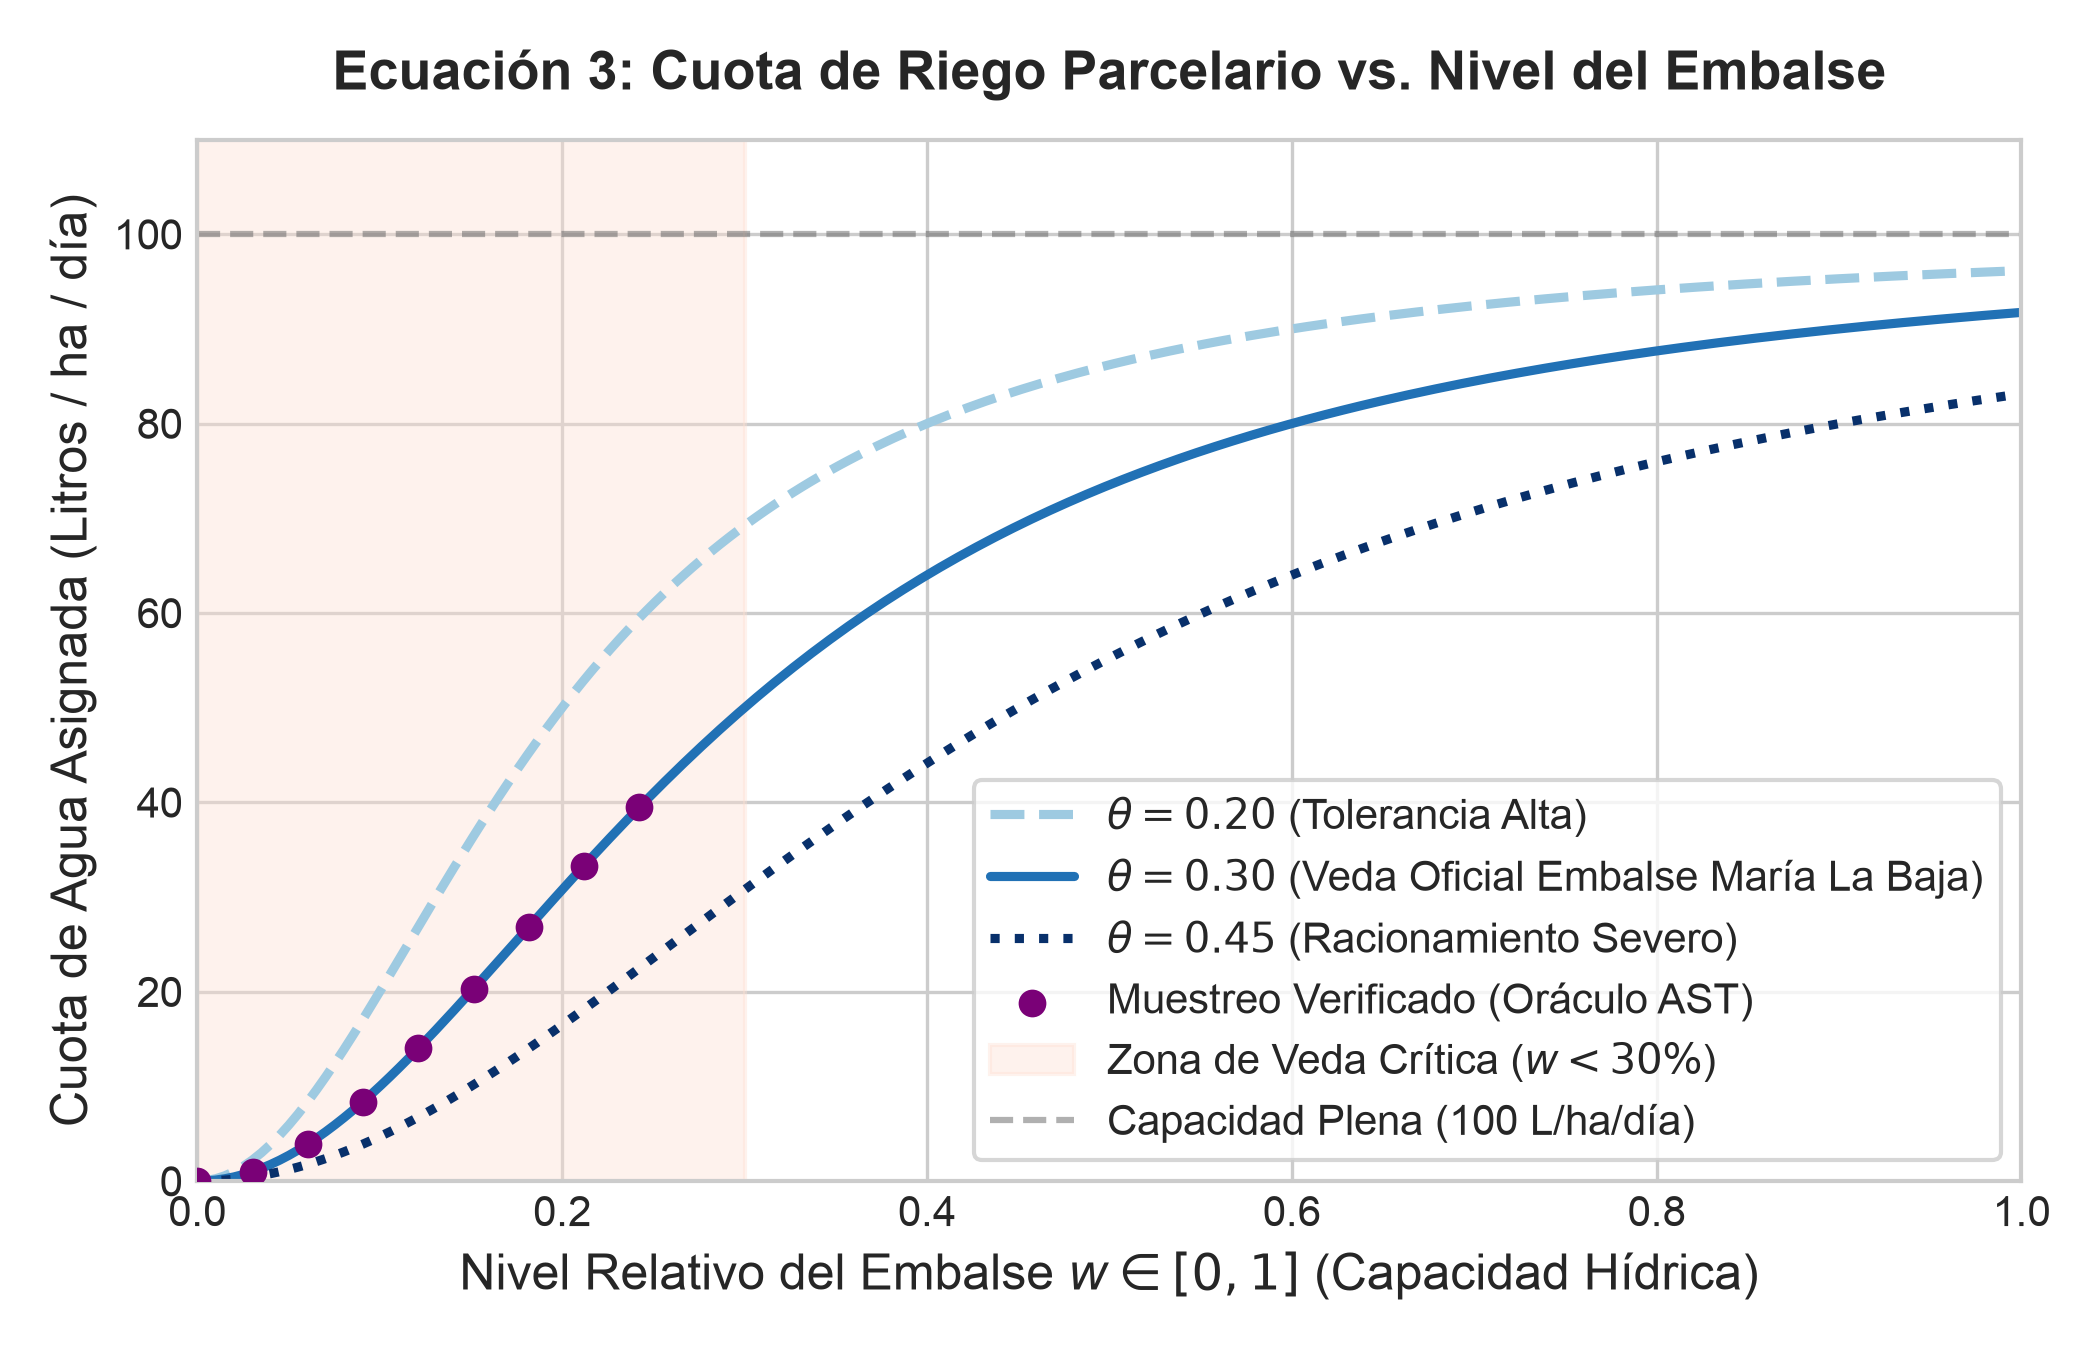
\includegraphics[width=0.78\textwidth]{../diagrams/out/fig_eq3_cuota_riego_reserva.png}
    \caption{Curva de cuota diaria de riego en funci\'on del nivel relativo del embalse, delimitando la zona de veda cr\'itica ($w < 30\%$) y la saturaci\'on de suministro.}
    \label{fig:eq3}
\end{figure}

% ==============================================================================
% 5. INTEGRACION Y EXPERIENCIA DE USUARIO (ATLAS UI)
% ==============================================================================
\section{Integraci\'on en la interfaz de usuario: consola interactiva de curadur\'ia}

Para facilitar la adopci\'on de este marco por el director e investigadores del proyecto, se enriqueci\'o la sub-vista agron\'omica del componente React / TypeScript \texttt{AtlasView.tsx}:

\begin{itemize}[leftmargin=*]
    \item \textbf{Consola de Ecuaciones Simb\'olicas:} Se incorpor\'o una pesta\~na dedicada denominada \textit{``Laboratorio de Ecuaciones Simb\'olicas Institucionales (Semana 11 - B7)''}, con un selector por botones para alternar entre las tres f\'ormulas validadas (\textit{Eq 1: Cr\'edito FINAGRO}, \textit{Eq 2: Precio Sustentaci\'on}, \textit{Eq 3: Cuota Riego}).
    \item \textbf{Control Deslizante Interactivo en Tiempo Real:} El investigador puede manipular mediante un control deslizante (\textit{slider}) continuo las variables de entrada ($S_{\text{social}}$, $Y_{\text{rel}}$, $w$) y observar de forma inmediata el c\'alculo resultante y su texto explicativo.
    \item \textbf{Insignias Din\'amicas de Auditor\'ia Formal:} Cuatro insignias visuales certifican en tiempo real los cuatro pilares del or\'aculo determinista: \textit{Monoton\'ia Conforme}, \textit{Rango V\'alido}, \textit{Cero Singularidades} y \textit{Seguridad AST Aprobada}.
    \item \textbf{Trazabilidad de Entidad y Estrato:} Cada ecuaci\'on visualiza claramente su estrato institucional (\texttt{institutional\_policy}) y la entidad receptora en EthosTerra (\texttt{BankOffice}, \texttt{MarketPlace}, \texttt{AgroEcosystem}).
\end{itemize}

% ==============================================================================
% 6. ARQUITECTURA DEL ADAPTADOR DESACOPLADO
% ==============================================================================
\section{Arquitectura del adaptador desacoplado de simulaci\'on}

La clase \texttt{EthosTerraDecoupledAdapter} materializa el principio de soberan\'ia e inmutabilidad del simulador:
\begin{itemize}[leftmargin=*]
    \item Escribe exclusivamente en la carpeta de sandbox \texttt{outputs/simulation\_sandbox/}, garantizando cero mutaciones en el repositorio \texttt{EthosTerra}.
    \item Compila \texttt{world\_modifiers.json}, consolidando las pol\'iticas que afectan las entidades bancarias, de mercado y ambientales.
    \item Emite \texttt{bundle\_manifest.json}, certificando el hash SHA-256 de cada archivo compilado, la identidad del investigador curador y los sellos de tiempo UTC.
\end{itemize}

% ==============================================================================
% 7. EVIDENCIA EMPIRICA Y PRUEBAS
% ==============================================================================
\section{Evidencia emp\'irica y resultados de pruebas}

La suite de pruebas automatizadas del monorepo fue expandida hasta alcanzar 278 casos de prueba rigurosamente aprobados (\texttt{make test-unit}):

\begin{table}[H]
\centering
\small
\caption{Resultados cuantitativos de la bater\'ia de pruebas unitarias.}
\label{tab:pruebas}
\begin{tabularx}{\textwidth}{lp{6.0cm}rX}
\toprule
\textbf{M\'odulo de Prueba} & \textbf{Alcance Evaluado} & \textbf{Casos} & \textbf{Estado} \\
\midrule
\texttt{test\_symbolic\_equation\_verifier.py} & Seguridad AST, inyecci\'on, monoton\'ia, singularidades & 13 & 100\% Aprobado \\
\texttt{test\_institutional\_schemas\_*.py} & Pydantic V2, tipolog\'ia institucional, compilaci\'on & 6 & 100\% Aprobado \\
\texttt{test\_ethosterra\_decoupled\_adapter.py} & Bundle sandbox, world\_modifiers, endpoints API & 5 & 100\% Aprobado \\
Suites heredadas Semanas 5--10 & Canario DMR, Caso Puro, Conflictivo, CRUD, Auth & 254 & 100\% Aprobado \\
\midrule
\textbf{Total general} & \textbf{Cobertura integral del monorepo} & \textbf{278} & \textbf{278/278 (100\%)} \\
\bottomrule
\end{tabularx}
\end{table}

Asimismo, la construcci\'on del frontend React TypeScript se ejecut\'o en 350\,ms sin advertencias de tipado:
\begin{lstlisting}[language=bash, caption={Reporte de compilaci\'on limpia del frontend.}]
> frontend@0.0.0 build
> tsc -b && vite build

dist/index.html                                  0.47 kB | gzip:   0.30 kB
dist/assets/maplibre-gl-worker-VaXr2Fck.mjs    508.31 kB
dist/assets/index-DAotwnwW.css                 158.46 kB | gzip:  24.17 kB
dist/assets/index-CLOgv-g6.js                1,748.94 kB | gzip: 466.00 kB
built in 350ms (cero errores de TypeScript)
\end{lstlisting}

% ==============================================================================
% 8. REPRODUCCION TECNICA
% ==============================================================================
\section{Comandos de reproducci\'on}

\begin{lstlisting}[language=bash, caption={Instrucciones de verificaci\'on local.}]
# 1. Ejecutar las 278 pruebas unitarias
make test-unit

# 2. Re-generar las figuras cientificas
uv run --with matplotlib --with numpy --with pydantic python scripts/generate_scientific_plots.py

# 3. Compilar el frontend
pnpm --dir apps/ui build
\end{lstlisting}

% ==============================================================================
% 9. REFERENCIAS BIBLIOGRAFICAS
% ==============================================================================
\section{Referencias}
\begin{enumerate}[leftmargin=*]
    \item Agencia de Renovaci\'on del Territorio (ART). (2019). \textit{Plan de Acci\'on para la Transformaci\'on Regional (PATR) -- Subregi\'on Montes de Mar\'ia}. Presidencia de la Rep\'ublica de Colombia, Bogot\'a D.C.
    \item Allen, R. G., Pereira, L. S., Raes, D., \& Smith, M. (1998). \textit{Crop evapotranspiration: Guidelines for computing crop water requirements}. FAO Irrigation and Drainage Paper No. 56, Food and Agriculture Organization of the United Nations, Roma.
    \item Bratman, M. E. (1987). \textit{Intentions, Plans, and Practical Reason}. Harvard University Press, Cambridge, MA.
    \item Congreso de la Rep\'ublica de Colombia. (2020). \textit{Ley 2046 de 2020: Por la cual se establecen mecanismos para promover la participaci\'on de peque\~nos productores locales agropecuarios en los mercados de compras p\'ublicas de alimentos}. Diario Oficial No. 51.417, Bogot\'a D.C.
    \item Departamento Administrativo Nacional de Estad\'istica (DANE). (2024). \textit{Marco Geoestad\'istico Nacional (MGN) y Codificaci\'on DIVIPOLA}. DANE, Bogot\'a D.C.
    \item Ortony, A., Clore, G. L., \& Collins, A. (1988). \textit{The Cognitive Structure of Emotions}. Cambridge University Press, Cambridge.
    \item Ostrom, E. (1990). \textit{Governing the Commons: The Evolution of Institutions for Collective Action}. Cambridge University Press, Cambridge.
    \item Rao, A. S., \& Georgeff, M. P. (1995). \textit{BDI agents: from theory to practice}. En Proceedings of the First International Conference on Multi-Agent Systems (ICMAS-95), pp. 312--319.
\end{enumerate}

\end{document}
